%# -*- coding: utf-8-unix -*-
% !TEX program = xelatex
% !TEX root = ../thesis.tex

\chapter{User Models}

    The training process of a reinforcement learning involves frequent interaction
    between the reinforcement learning agent and users.
    Deploying an unreliable reinforcement learning algorithm in production is not a feasible option.
    On one hand, the agent is not well-trained, producing bad or misleading recommendations,
    which could jeopardize the education process.
    On the other hand, a single interaction between the agent and the student takes a long time.
    It takes hours if not days for a student to solve a problem,
    not to mention the even longer interval before attempting another problem.
    Hence, it could take tens of years to train the agent if not impossible at all.

    Therefore, we developed another approach.
    We firstly trained a \emph{user model} to capture students' mindsets using the existing submission records.
    Then, we programmed the reinforcement learning to interact with the user model.
    This real-time interaction enabled the successful training process.

    \todo{chapter overview}

\section{Problem Formulation}

    We formulate the user model as a binary classifier:
    given the user features, problem features, and the context features,
    the user model predicts whether the user is able to solve the problem,
    more precisely,
    it is the probability of the user able to solve the problem that we care about.

    The training and validation data is from the submission records of the Online Judge.
    We used the earliest 80\% records as the training set,
    and the most recent 20\% records is the validation set.
    For each submission record, the user features and the context features
    count statistics before the user made this submission.
    On the other side, we believe that the objective difficulty of each problem should not change over time.
    Hence, the more records are used, the better the generated problem features estimate the objective difficulty.
    Therefore, the problem features are the exactly the same for the same problem,
    generated using all of the submissions.

\section{Backgrounds}

    \subsection{Feature Scaling}

        The range of features in our feature set varies a lot.
        For example, $\verb|uf_ac_rate| \in [0,1]$, but $\verb|uf_avg_bytes|$ can be a few thousands.

        Feature scaling is a method to standardize the range of independent variables or features of data,
        making the learning process more robust.
        Another reason is that stochastic gradient decent converges much faster with feature scaling than without it.
        \cite{ioffe_batch_2015}

        We scaled each feature to $[0,1]$ in the following manner before feeding the input matrix $X$ to a user model.
        \[
        X_{:,j} \leftarrow \frac{X_{:,j}}{\max X_{:,j}}
        \]

        Notice that, not every user model is sensitive to feature scaling.
        For example, feature scaling has no effect on the boosted trees, because they deal with discrete values.

    \subsection{Metrics: Accuracy and AUC}

        To have a sense of the performance of a user model, we watch the following two metrics:
        classification accuracy and AUC.

        Classification accuracy, as the name suggests, is the ratio of
        the number of correct predictions to the total number of predictions made.
        A overfitted model tend to have a big gap between the train accuracy and the validation accuracy.

        Area under the receiver operating characteristic curve (\emph{AUC})
        is another most widely used metrics in classification tasks.
        There can be several equivalent interpretations of AUC \cite{flach_putting_2007}:

        \begin{itemize}
            \item The expectation that a uniformly drawn random positive is ranked before a uniformly drawn random negative.
            \item The expected proportion of positives ranked before a uniformly drawn random negative.
            \item The expected true positive rate if the ranking is split just before a uniformly drawn random negative.
            \item The expected proportion of negatives ranked after a uniformly drawn random positive.
            \item 1 – the expected false positive rate if the ranking is split just after a uniformly drawn random positive.
        \end{itemize}


\section{Logistic Regression}

    Tom Mitchell gives a formal definition of machine learning:
    ``A computer program is said to learn from experience $E$ with respect to some class of tasks $T$
    and performance measure $P$ if its performance at tasks in $T$, as measured by $P$, improves with experience $E$.''
    \cite{Mitchell1997}
    Machine learning relies on experience.
    Depending on what experience is like, machine learning tasks can be broadly classified into two types:
    supervised learning and unsupervised learning.

    A supervised learning task learns a function based on example training data.
    In supervised learning, each piece of training data consist of a pair of input vector
    and the desired output, called \emph{label}.
    A supervised learning algorithm goes through the training data and infers the function
    which can be used to predict new examples.
    In contrast to the performance on the training data,
    researchers pay more attention to the ability of the model to correctly predict unseen data,
    i.e. the capability of generalization.
    Sometimes, predictions on the input training data can greatly outperform that on unseen data.
    In this case, the model is overfitted, meaning that the model has ``memorized'' the training data
    but did not ``learn''.

    Logistic regression is a widely used supervised learning model.
    The output of logistic regression is a probability for a label to belong to a given data.
    The label is binary discrete.
    In other words, a data point can only be either a positive sample or a negative sample.
    Given input vector $x$ and some coefficients $w$,
    logistic regression learns a function of the following form:

    \begin{align*}
        P(y=1 | x;w) &= \frac{1}{1+\exp(-w^Tx)} = \sigma(w^Tx)\\
        P(y=0 | x;w) &= 1-P(y=1 | x) = 1-\sigma(w^Tx)
    \end{align*}

    where

    \[
    \sigma(x) = \frac{1}{1+\exp(-z)}
    \]

    is the logistic function (or the \emph{sigmoid} function).
    It is an ``S''-shaped function, mapping $w^Tx$ to $[0,1]$
    so that we can interpret $\sigma(w^Tx)$ as a probability.
    Training a logistic regression model is a process that tries to find $w$ so that
    $P(y=1 | x)$ is large for the input vector $x$ that belongs to the positive class,
    and symmetrically, $P(y=0 | x)$ is large for the input vector $x$ that belongs to the negative class.

    For a set of training examples with binary labels $\left\{ (x^{(i)}, y^{(i)} | i = 1, 2, \cdots, m) \right\}$,
    the loss function, i.e. the log likelihood, is

    \[
    l(w) = -\sum_{i=1}^m \left( y^{(i)}\log\left(\sigma(w^Tx^{(i)})\right) + (1-y^{(i)})\log\left(1-\sigma(w^Tx^{(i)})\right) \right)
    \]

    It can be prove \cite{Ng2000} that the gradient of the loss function is

    \[
    \nabla_w l(w) = \sum_{i=1}^m x^{(i)}\left(\sigma(w^Tx^{(i)}) - y^{(i)}\right)
    \]

    We can derive the update rule of the stochastic gradient ascent from this:

    \[
    w_j := w_j + \eta \left( y^{(i)} - \sigma(w^Tx^{(i)}) \right) x_j^{(i)}
    \]

    where $\eta$ is the learning rate.

    In other words, the computation of both the logistic regression model and its gradient is fast.
    Consequently, logistic regression model is widely adopted in the industry,
    especially where computation time is limited, such as click-through-rate estimation \cite{DBLP:journals/corr/WangZY16}
    and recommendation systems.

    \subsection{Kernel Tricks}

        The definition of logistic regression shows that it's a linear model
        because the relation of the input vector $x$ and the coefficients $w$ is a linear combination.
        However, the capability of a linear model is limited.
        It cannot discover the relationship between different input features,
        i.e., different dimensions of the input vector.

        For instance, in a recommendation system, there is usually three types of features: \cite{Ricci2011}

        \begin{description}
            \item[User Features] Each user may have a set of attributes.
                For example, user demographic includes users' age, gender, and so on.
                Some of these features may be filled by the user, like education level.
                And others can be inferred by their behavior, such as their interested music genres.
            \item[Item Features] Items are products which the recommendation system would like to recommend to users,
                such as books on an online shop.
                Items also have a set of characteristics.
                For example, the author of a book.
            \item[Context Features] These features reflects interactions between users and items.
                Some features provide additional information,
                for example, it can be it can be a user's rate on a specific book.
                Others can be derived from user features and item features.
        \end{description}

        To enable a linear model to capture the relations between user features and item features,
        it requires domain experts manually calculating context features.

        Mathematically, the data points are not always linearly separable.
        Kernel tricks enables linear models like logistic regression to capture non-linear regression.

        For all $x$ and $x'$ in the input space $\mathcal{X}$,
        certain functions $k(x, x')$ can be expressed as an inner product $\langle\cdot,\cdot\rangle_{\mathcal{V}}$
        in another space $\mathcal{V}$:

        \[
        k(x, x') = \langle \varphi(x), \varphi(x') \rangle_{\mathcal{V}}
        \]

        where $\varphi: \mathcal{X} \rightarrow \mathcal{V}$ is the feature map.
        The function $k: \mathcal{X} \times \mathcal{X} \rightarrow \mathbb{R}$ is called a \emph{kernel} function.

        For example, consider a two dimension space.
        Data points $(x_1, x_2)$ within a oval are positive samples and others are negative samples
        (See Figure \ref{fig:kernel-tricks}).
        In this case, it is not linear separable.
        Consider the feature map $\varphi((x_1, x_2)) = (x_1^2, \sqrt{2}x_1x_2, x_2^2)$.
        Now data becomes linearly separable. \cite{Rai2011}

        \begin{figure}[!htp]
            \centering
            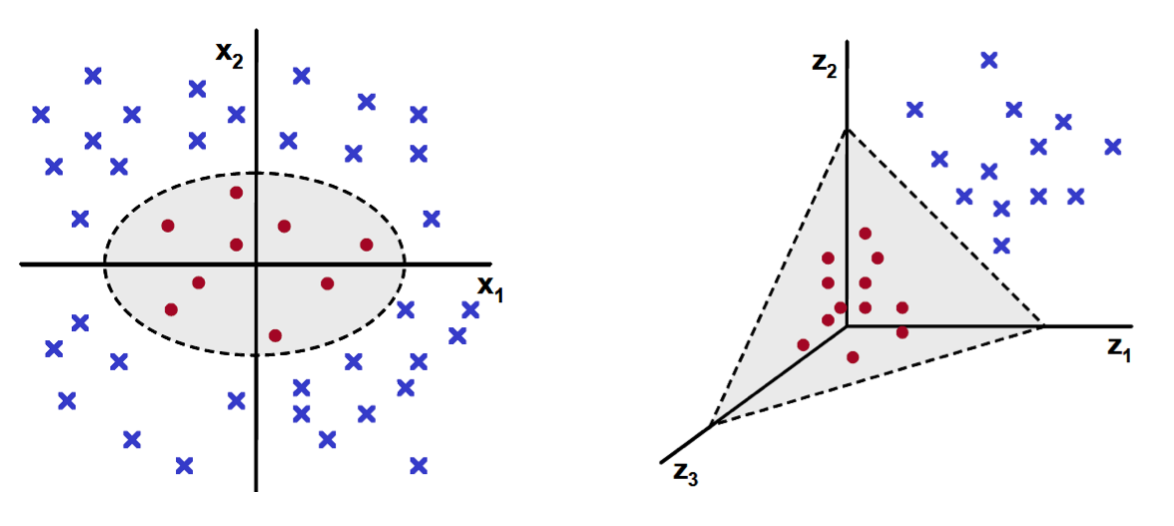
\includegraphics[width=0.62\textwidth]{img/kernel-tricks.png}
            \caption{Transforming a set of non-linearly separable data points to a linearly separable one.
                Credit to the figure: \textcite{Rai2011}.}
            \label{fig:kernel-tricks}
        \end{figure}

        The more general kernel is quadratic kernels.
        Consider data point $x = (x_1, x_2, \cdots, x_n)$.
        A quadratic kernel maps $x$ to 

        \[
        \varphi(x) := (1, \sqrt{2}x_1, \cdots, \sqrt{2}x_n, x_1^2, \cdots, x_n^2,
          \sqrt{2}x_1x_2, \cdots, \sqrt{2}x_1x_n, \cdots, \sqrt{2}x_{n-1}x_n)
        \]

        Each new feature uses a pair of the original features,
        therefore, it can capture the interaction between each pair of features.

\section{Factorization Machine}

    \subsection{Limitation of Kernel Tricks}

        Notice that, the linear combination of the transformed feature vector and the coefficients is

        \[
        w^T\varphi(x) = w_0 + \sqrt{2}\sum_{i=1}^n w_ix_i
        + \sum_{i=1}^n w_{ii}x_i^2 + \sqrt{2}\sum_{i=1}^n\sum_{j=i+1}^n w_{ij}x_ix_j
        \]

        In other words, the number of parameters of a $n$-dimension input has $O(n^2)$ dimensions.
        However, it may not work well with recommendation systems.

        The input vector of recommendation systems are usually sparse.
        For example, there can be some one-hot features.
        A one-hot feature may span thousands of dimension.
        There is only one dimension has non-zero value and the others are all zeros.

        The blast of the number of parameters makes the training process inefficient.
        What's worse, in order to learn $w_{ij}$,
        there need to be enough input vectors that satisfy $x_i \neq 0$ and $x_j \neq 0$,
        which usually is not true for all pairs of $i$ and $j$.
        Consequently, the inefficient learning process might eventually result in a ineffective model
        because $w_{ij}$ is noisy.
        It is obvious that this issue will become worse if we want to capture relations of three or more features.

    \subsection{Factorization Machine}

        Factorization machine allows parameter estimation under very sparse data
        where linear regressions with kernel tricks fail. \cite{Rendle2010}

        The model equation for a factorization machine of degree $d=2$ is defines as:

        \begin{equation}
        y(x) := w_0 + \sum_{i=1}^n w_i x_i + \sum_{i=1}^n\sum_{j=i+1}^n \langle \bm{v}_i, \bm{v}_j \rangle x_ix_j
        \label{eq:fm}
        \end{equation}

        where the the model parameters that have to be estimated are:

        \[
        w_0 \in \mathbb{R}, \quad w \in \mathbb{R}^n, \quad \bm{V} \in \mathbb{R}^{n \times k}
        \]

        And $\langle \cdot, \cdot \rangle$ is the dot product of two vectors of size $k$:

        \[
        \langle \bm{v}_i, \bm{v}_j \rangle := \sum_{f=1}^k v_{if}v_{jf}
        \]

        A row $\bm{v}_i$ within $\bm{V}$ describes the $i$-th variable with $k$ factors.
        $k \in \mathbb{N}_0^+$ is a hyperparameter that defines the dimensionality of the factorization.

        The two-degree factorization machine captures all single and pairwise interactions between variables:

        \begin{itemize}
            \item $w_0$ is the global bias.
            \item $w_i$ models the importance of $i$-th variable.
            \item $\langle \bm{v}_i, \bm{v}_j \rangle$ reflects the interaction
                between the $i$-th variable and the $j$-th variable.
        \end{itemize}

        The difference between the factorization machine and kernel tricks is that
        kernel tricks use a independent parameter for each pair of interaction, resulting in $O(n^2)$ parameters,
        but the factorization machine models the interaction by factorizing it, resulting in $O(nk)$ parameters.
        For large enough $k$, the factorization machine is able to express any interaction matrix $\bm{W}$ \cite{Rendle2010},
        therefore, the factorization machine is as expressive as kernel tricks.
        On the other hand, choosing small $k$ restricts the capability of the factorization machine,
        which in turn can reduce the noisy and leads to better generalization under sparsity,
        because there is not enough data to disclose the complicated pairwise interaction.

        Although the complexity of calculating the score function of the factorization machine \ref{eq:fm}
        might seem to be $O(kn^2)$ if taking a naive approach,
        transforming the formula in the following manner shows that it can be done in linear time $O(kn)$:

        \begin{align*}
        & \sum_{i=1}^n\sum_{j=i+1}^n \langle \bm{v}_i, \bm{v}_j \rangle x_ix_j \\
        =& \frac { 1} { 2} \sum _ { i = 1} ^ { n } \sum _ { j = 1} ^ { n } \left\langle \bm { v } _ { i } ,\bm { v } _ { j } \right\rangle x _ { i } x _ { j } - \frac { 1} { 2} \sum _ { i = 1} ^ { n } \left\langle \bm { v } _ { i } ,\bm { v } _ { i } \right\rangle x _ { i } x _ { i } \\
        =& \frac { 1} { 2} \left( \sum _ { i = 1} ^ { n } \sum _ { j = 1} ^ { n } \sum _ { f = 1} ^ { k } v _ { if } v _ { jf} x _ { i } x _ { j } - \sum _ { i = 1} ^ { n } \sum _ { f = 1} ^ { k } v _ { if } v _ { if } x _ { i } x _ { i } \right) \\
        =& \frac { 1} { 2} \sum _ { f = 1} ^ { k } \left( \left( \sum _ { i = 1} ^ { n } v _ { if } x _ { i } \right) \left( \sum _ { j = 1} ^ { n } v _ { jf } x _ { j } \right) - \sum _ { i = 1} ^ { n } v _ { if } ^ { 2} x _ { i } ^ { 2} \right) \\
        =& \frac { 1} { 2} \sum _ { f = 1} ^ { k } \left( \left( \sum _ { i = 1} ^ { n } v _ { if } x _ { i } \right) ^ { 2} - \sum _ { i = 1} ^ { n } v _ { if } ^ { 2} x _ { i } ^ { 2} \right)
        \end{align*}

        The two-degree factorization machine can be generalized to a $d$-degree factorization machine:

        \[
        y(x) = w_0 + \sum_{i=1}^n w_ix_i +
        \sum_{l=2}^d\sum_{i_1=1}^n\cdots\sum_{i_{l-1}+1}^n \left( \prod_{j=1}^l x_{i_j} \right)
        \left( \sum_{f=1}^{k_l}\prod_{j=1}^l v_{i_j,f}^{(l)} \right)
        \]

        where the interaction parameters for the $l$-th interaction is

        \[
        \bm{V}^{(l)} \in \mathbb{R}^{n \times k_l}, \quad k_l \in \mathbb{N}_0^+
        \]

        It can be proved that by similar transformation, the computation is still linear. \cite{Rendle2010}

        To sum up, the factorization machine is an efficient algorithm
        that can capture interactions of two or more variables
        and has better generalization under sparsity compared to kernel tricks.

    \subsection{Implementation}

        We used the \verb|fastFM|\cite{bayer_fastfm:_2016} Python library.
        We chose the stochastic gradient descent solver with the hyper-parameters shown in Table \ref{table:fm param}.

        \begin{table}[hpbt]
        \centering
        \begin{tabular}{lcl}
            \hline
            Hyper-parameter & Value & Description \\
            \hline
            \verb|n_iter|    & 100,000 & The number of iterations of individual samples. \\
            \verb|init_std|  & 0.1 & The standard deviation for the initialization of the parameters. \\
            \verb|rank|      & 2 & The rank of the factorization used for the second order interactions. \\
            \verb|l2_reg_w|  & 0 & L2 penalty weight for linear coefficients. \\
            \verb|l2_reg_V|  & 0 & L2 penalty weight for pairwise coefficients. \\
            \verb|l2_reg|    & 0 & L2 penalty weight for all coefficients. \\
            \verb|step_size| & 0.001 & Step size for the SGD solver. \\
            \hline
        \end{tabular}
        \caption{The hyper-parameters of the factorization machine user model}
        \label{table:fm param}
        \end{table}

    \subsection{Result}

        Table \ref{table:fm result} shows the validation result of the factorization machine user model.

        \begin{table}[hpbt]
        \centering
        \begin{tabular}{lll}
            \hline
            Feature Set & Accuracy & AUC \\
            \hline
            Basic    & \verb|0.6877472027750164| & \verb|0.6835856799533652| \\
            Extended & \verb|0.6936271917764758| & \verb|0.6580982070227229| \\
            \hline
        \end{tabular}
        \caption{The result of the factorization machine user model}
        \label{table:fm result}
        \end{table}

\section{Boosted Tree}

        Decision tree is another widely used model for data analysis.

        A decision tree is a binary tree.
        Each node has exactly one parent (except for the only root node) and two children.
        Each internal node split the input subspace into two halves by a certain criteria.
        The leaves represents a category.

        Given a decision tree, the evaluation of a input is quite straight forward.
        At each internal node, decide which children to go by check the criteria.
        Repeat the procedure above recursively until reaching a leaf node.

        Similarly, the interpretation of a decision tree is also straight forward,
        which is its unique advantage over other machine learning algorithms.
        Because each node has a certain criteria,
        drawing the binary tree along with those criteria would give a clear explanation.
        A data analysis service provider can explain the model to the buyer by visualizing
        the decision tree without the need for the buyer to know statistic or machine learning knowledge.

    \subsection{XGBoost}

        Gradient boosting is a machine learning technique,
        which produces a prediction model in the form of an ensemble of weak prediction models.
        Gradient boosting is typically used with decision trees of a fixed size as base learners.
        For this special case, \cite{Friedman2001} proposes a modification to gradient boosting method
        which improves the quality of fit of each base learner.

        XGBoost is a scalable machine learning system for tree boosting. \cite{Chen2016}

    \subsection{Implementation}

        We used the \verb|xgboost|\cite{Chen2016} Python library
        with the hyper-parameters shown in Table \ref{table:xgboost param}.

        \begin{table}[hpbt]
        \centering
        \begin{tabular}{lcl}
            \hline
            Hyper-parameter & Value & Description \\
            \hline
            \verb|booster| & gbtree & We use gradient boosting tree as the booster method. \\
            \verb|num_boost_round| & 10 & The number of boosting iterations. \\
            \verb|max_depth| & 7 & Maximum tree depth for base learners. \\
            \verb|learning_rate| & 0.3 & Boosting learning rate. \\
            \hline
        \end{tabular}
        \caption{The hyper-parameters of the boosted tree user model}
        \label{table:xgboost param}
        \end{table}

    \subsection{Result}

        Table \ref{table:fm result} shows the validation result of the boosted tree user model.

        \begin{table}[hpbt]
        \centering
        \begin{tabular}{lll}
            \hline
            Feature Set & Accuracy & AUC \\
            \hline
            Basic    & \verb|0.7029230736690708| & \verb|0.7104618544225273| \\
            Extended & \verb|0.7184056346369424| & \verb|0.7352554610590846| \\
            \hline
        \end{tabular}
        \caption{The result of the boosted tree user model}
        \label{table:xgboost result}
        \end{table}

\section{Recurrent Neural Networks}

    Recurrent neural networks are a family of neural networks for processing sequential data.
    Traditional neural networks assumes the inputs are independent of each other,
    thus they cannot find connections inside the input of sequential data.
    In order to process sequential data, the model need to know context information.
    For example, predicting the next character in a sentence would heavily depend on
    characters came before it.

    Recurrent neural networks ``recurrently'' compute the output of current step
    depending on the calculation of the previous step.
    In other words, recurrent neural networks have internal states
    that memorize the context information between steps.

    \subsection{Vanilla Recurrent Neural Networks}

        \begin{figure}[!htp]
            \centering
            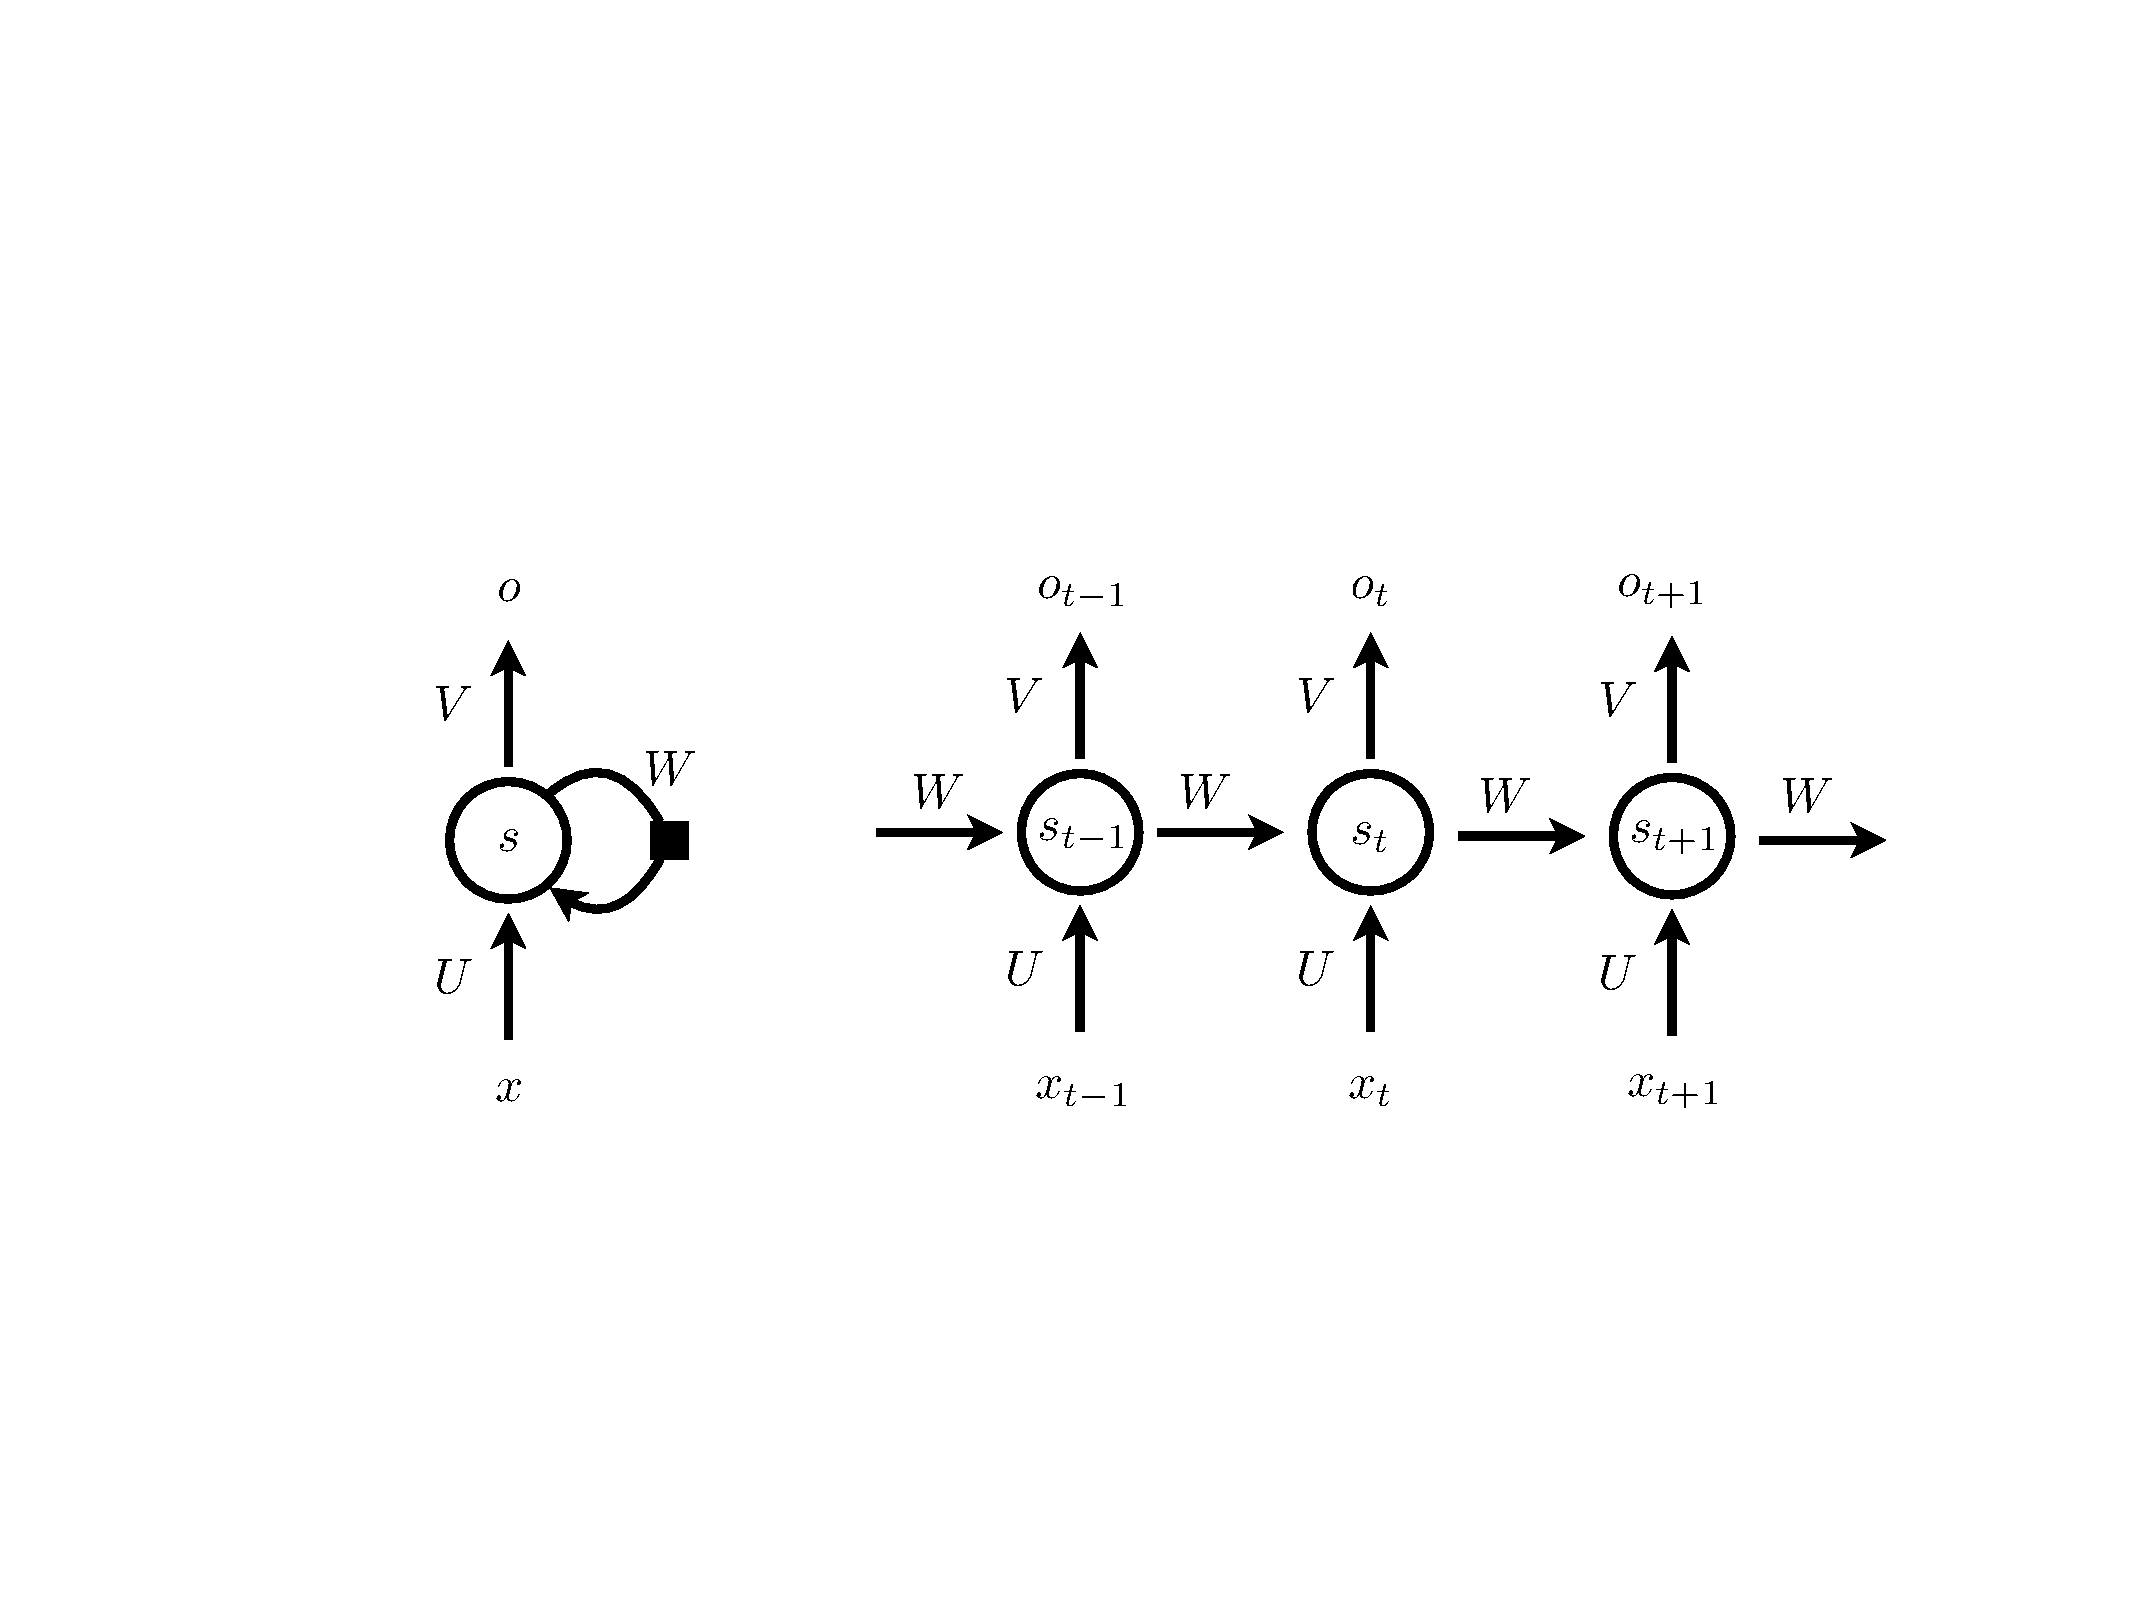
\includegraphics[width=0.62\textwidth]{img/rnn.pdf}
            \caption{Unfolding of the vanilla recurrent neural network}
            \label{fig:rnn}
        \end{figure}

        Figure \ref{fig:rnn} shows the unfold of the vanilla recurrent neural network.

        \begin{itemize}
            \item $x_t$ is the input at time step $t$.
                Interestingly, inputs may not be needed for each time step.
                For instance, in the image captioning task,
                the input presents only at the first time step which is the input image.
                The recurrent neural network then produce the sentence step by step and character by character.
            \item $h_t$ is the hidden state at time step $t$.
                Its computation depends on the previous hidden state and input of the current time step:
                $h_t = f(Ux_t + Wh_{t-1})$.
                Thus, it memorizes the context until so far.
                The activation function $f$ is usually a nonlinear function like $\tanh$ or $\mathrm{ReLU}$,
                which gives the recurrent neural network the capability of fitting a nonlinear function.
                The initial state $h_0$ is usually initialized to all zeros.
            \item $o_t$ is the output at time step $t$.
                For binary classification, it would be the sigmoid function $o_t = \sigma(Vh_t)$.
                Depending on the task, the output does not necessarily present in every time step.
                For example, determining the sentiment of a sentence only cares about the final output.
                On the other hand, predicting a sentence character by character would need outputs at all time steps.
            \item Unlike traditional neural networks,
                all time steps share the same parameters $U$, $V$, and $W$ in recurrent neural networks.
        \end{itemize}

        In theory, recurrent neural networks has the capability to handle arbitrarily long sequences.
        However, in practice, vanilla recurrent neural networks do not seem to be able to learn them.
        \cite{Pascanu2013}

    \subsection{Long Short Term Memory Networks}

        Long Short Term Memory networks (\emph{LSTM}) are a special kind of recurrent neural networks.
        It is capable of learning long-term dependencies.
        In addition to the input vector, the output vector, and the hidden state,
        it consists of three additional gates: the input gate, the output gate, and the forgot gate.
        More formally,

        \begin{align*}
            f_t &= \sigma_g(W_fx_t + U_fh_{t-1} + b_f) \\
            i_t &= \sigma_g(W_ix_t + U_ih_{t-1} + b_i) \\
            o_t &= \sigma_g(W_ox_t + U_oh_{t-1} + b_o) \\
            c_t &= f_t \odot c_{t-1} + i_t \odot \sigma_c(W_cx_t + U_ch_{t-1} + b_c) \\
            h_t &= o_t \odot \sigma_h(c_t)
        \end{align*}

        Meanings of the variables are the following:

        \begin{itemize}
            \item $x_t \in \mathbb{R}^d$: The input vector
            \item $f_t \in \mathbb{R}^h$: The forget gate's activation vector
            \item $i_t \in \mathbb{R}^h$: The input gate's activation vector
            \item $o_t \in \mathbb{R}^h$: The output gate's activation vector
            \item $h_t \in \mathbb{R}^h$: The output vector of the LSTM unitTh
            \item $c_t \in \mathbb{R}^h$: The cell state vector
            \item $W \in \mathbb{R}^{h \times d}, U \in \mathbb{R}^{h \times h}, b \in \mathbb{R}^{h}$: 
                The parameters
        \end{itemize}

        And the choices of activation functions:

        \begin{itemize}
            \item $\sigma_g$: the sigmoid function
            \item $\sigma_c$: the $\tanh$ function
            \item $\sigma_h$: the $\tanh$ function or the identity function $\sigma_h(x) = x$
        \end{itemize}

        The core idea behind LSTMs is to control how much of the information should go through. \cite{Ola2015}
        The cell state $c_t$ ``memorizes'' the context and flows along the time steps,
        adapting changes at each time step.
        Gates provide a way to optionally let information through.
        They are composed out of a sigmoid neural net layer and a element-wise multiplication operation.
        We can think of the sigmoid layer as controlling how much of the change should be let through.

    \subsection{Implementation}

        We use the \verb|Keras|\cite{chollet2015keras} Python library to build the neural network.
        The neural network consists of a LSTM layer and a fully connected layer.
        In addition to features at the current time step,
        the input vector also contains features of the user's five previous submissions ($\verb|lookback| = 5$)
        and whether those submissions were accepted.
        The output dimension of the LSTM layer is 10.
        The fully connected layer only has a scalar output activated by the sigmoid function.
        We use the Adam optimizer\cite{kingma_adam:_2014}.

    \subsection{Result}

        Table \ref{table:rnn result} shows the validation result of the recurrent neural network user model.

        \begin{table}[hpbt]
        \centering
        \begin{tabular}{lll}
            \hline
            Feature Set & Accuracy & AUC \\
            \hline
            Basic    & \verb|0.7163222572389433| & \verb|0.7232273437233644| \\
            Extended & \verb|0.7194526110958354| & \verb|0.7308123624422472| \\
            \hline
        \end{tabular}
        \caption{The result of the recurrent neural networks user model}
        \label{table:rnn result}
        \end{table}

\section{Counting Features}

    \todo{counting feature: count before vs. after}










